\documentclass[10pt]{article}
\usepackage[utf8]{inputenc}
\usepackage[english]{babel}
\usepackage[font=small,labelfont=bf]{caption}
\usepackage{geometry}
\usepackage[sort&compress, numbers]{natbib}
\usepackage{pxfonts}
\usepackage{graphicx}
\usepackage{setspace}
\usepackage{hyperref}
\usepackage{lineno}

% supplemental tables
\newcommand{\questions}{S1}

% supplemental figures



\doublespacing
\linenumbers

\title{Geometric models reveal the hidden structure of conceptual knowledge}

\author{Paxton C. Fitzpatrick and Jeremy R.
Manning\textsuperscript{*}\\Dartmouth
College\\\textsuperscript{*}Corresponding author:
jeremy.r.manning@dartmouth.edu}

\date{}

\begin{document}
\maketitle

\begin{abstract} We develop a mathematical framework, based on natural language
processing models, for tracking and characterizing the acquisition of
conceptual knowledge. Our approach embeds each concept in a high dimensional
representation space, where nearby coordinates reflect similar or related
concepts. We tested our approach using behavioral data collected from a group
of college students. In the experiment, we asked the participants to answer
sets of quiz questions interleaved between watching two course videos from the
Khan Academy platform. We applied our framework to the videos' transcripts, and
to text of the quiz questions, to quantify the content of each moment of video
and each quiz question. We used these embeddings, along with participants' quiz
responses, to track how the learners' knowledge changed after watching each
video. Our findings show how a limited set of quiz questions may be used to
construct rich and meaningful representations of what each learner knows, and
how their knowledge changes over time as they learn.

\textbf{Keywords: education, learning, knowledge, concepts, natural language processing}

\end{abstract}


\section*{Introduction}

How do we acquire conceptual knowledge? Memorizing course lectures or textbook
chapters by rote can lead to the superficial \textit{appearance} of
understanding the underlying content, but achieving true conceptual
understanding seems to require something deeper and richer. Does conceptual
understanding entail connecting newly acquired information to the scaffolding
of one's existing knowledge or experience~\citep{BlayEtal06,CaraMaho03,
ConsEtal16, DeacEtal04, SimoEtal04}? Or weaving a lecture's atomic
elements (e.g., its component words) into a structured network that describes
how those individual elements are related? Conceptual understanding could also
involve building a mental model that transcends the meanings of those
individual atomic elements by reflecting the deeper meaning underlying the
gestalt whole~\citep{Kint70, Macl05, ScotEtal07}.

The difference between ``understanding'' and ``memorizing,'' as framed by the
researchers in education, cognitive psychology, and cognitive
neuroscience~\citep{Kato40, Gall00, ScotEtal07, HallGree08, Macl05} has
profound analogs in the fields of natural language processing and natural
language understanding. For example, considering the raw contents of a document
(e.g., its constituent symbols, letters, and words) might provide some
information about what the document is about, just as memorizing a passage
might be used to answer simple questions about the passage~\citep[e.g., whether
it might contain words related to furniture versus physics;][]{LandDuma97,
BleiEtal03, BleiLaff06}. However, modern natural language processing
models~\citep[e.g.,][]{MikoEtal13a, CerEtal18, BrowEtal20} also attempt to
capture the deeper meaning \textit{underlying} those atomic elements. These
models consider not only the co-occurrences of those elements within and across
documents, but also patterns in how those elements appear across different
scales (e.g., sentences, paragraphs, chapters, etc.), the temporal and
grammatical properties of the elements, and other high-level characteristics of
how they are used~\citep{Mann20, Mann21a}. According to these models, the deep
conceptual meaning of a document may be captured by a feature vector in a
high-dimensional representation space, where nearby vectors reflect
conceptually related documents. A model that succeeds at capturing an analog of
``understanding'' is able to assign nearby feature vectors to two conceptually
related documents, \textit{even when the words contained in those documents
have very little overlap}.

What form might the representation of the sum total of a person's knowledge
take? First, we might require a means of systematically describing or
representing the nearly infinite set of possible things a person could know.
Second, we might want to account for potential associations between different
concepts. For example, the concepts of ``fish'' and ``water'' might be
associated in the sense that fish live in water. Third, knowledge may have a
critical dependency structure, such that knowing about a particular concept
might require first knowing about a set of other concepts. For example,
understanding the concept of a fish swimming in water first requires
understanding what fish and water \textit{are}. Fourth, as we learn, our
``current state of knowledge'' should change accordingly. Learning new concepts
should both update our characterizations of ``what is known'' and should also
unlock any now-satisfied dependencies of that newly learned concept so that
they are ``tagged'' as available for future learning.

Here we develop a framework for modelling how knowledge is acquired during
learning. The central idea is to use text embedding models to define the
coordinate systems of two maps: (a) a \textit{knowledge map} that describes the
extent to which each concept is currently known and (b) a \textit{learning map}
that describes the extent to which each concept could be learned. Each location
on these maps represents a single concept, and the geometries are defined such
that related concepts are located nearby in space. We use this framework to
analyzing and interpreting behavioral data collected from an experiment that
has participants watch and answer conceptual questions about a series of
recorded course lectures.

Our primary research goal is to advance our understanding of what it means to
acquire deep real-world conceptual knowledge. Traditional laboratory approaches
to studying learning and memory (e.g., list learning studies) often draw little
distinction between memorization and understanding. Instead, these studies
typically focus on whether information is effectively encoded or retrieved,
rather than whether the information is \textit{understood}. Approaches to
studying conceptual learning, such as category learning experiments, can start
to investigate the distinction between memorization and understanding, often by
training participants to distinguish arbitrary or random features in otherwise
meaningless categorized stimuli. However the objective of real-world training,
or learning from life experiences more generally, is often to develop new
knowledge that may be applied in \textit{useful} ways in the future. In this
sense, the gap between modern learning theories and modern pedagogical
approaches and classroom learning strategies is enormous: most of our theories
about \textit{how} people learn are inspired by experimental paradigms and
models that have only peripheral relevance to the kinds of learning that
students and teachers actually seek. To help bridge this gap, our study uses
course materials from real online courses to inform, fit, and test models of
real-world conceptual learning.

\section*{Results}

% \begin{figure}[tp]
% \centering
% 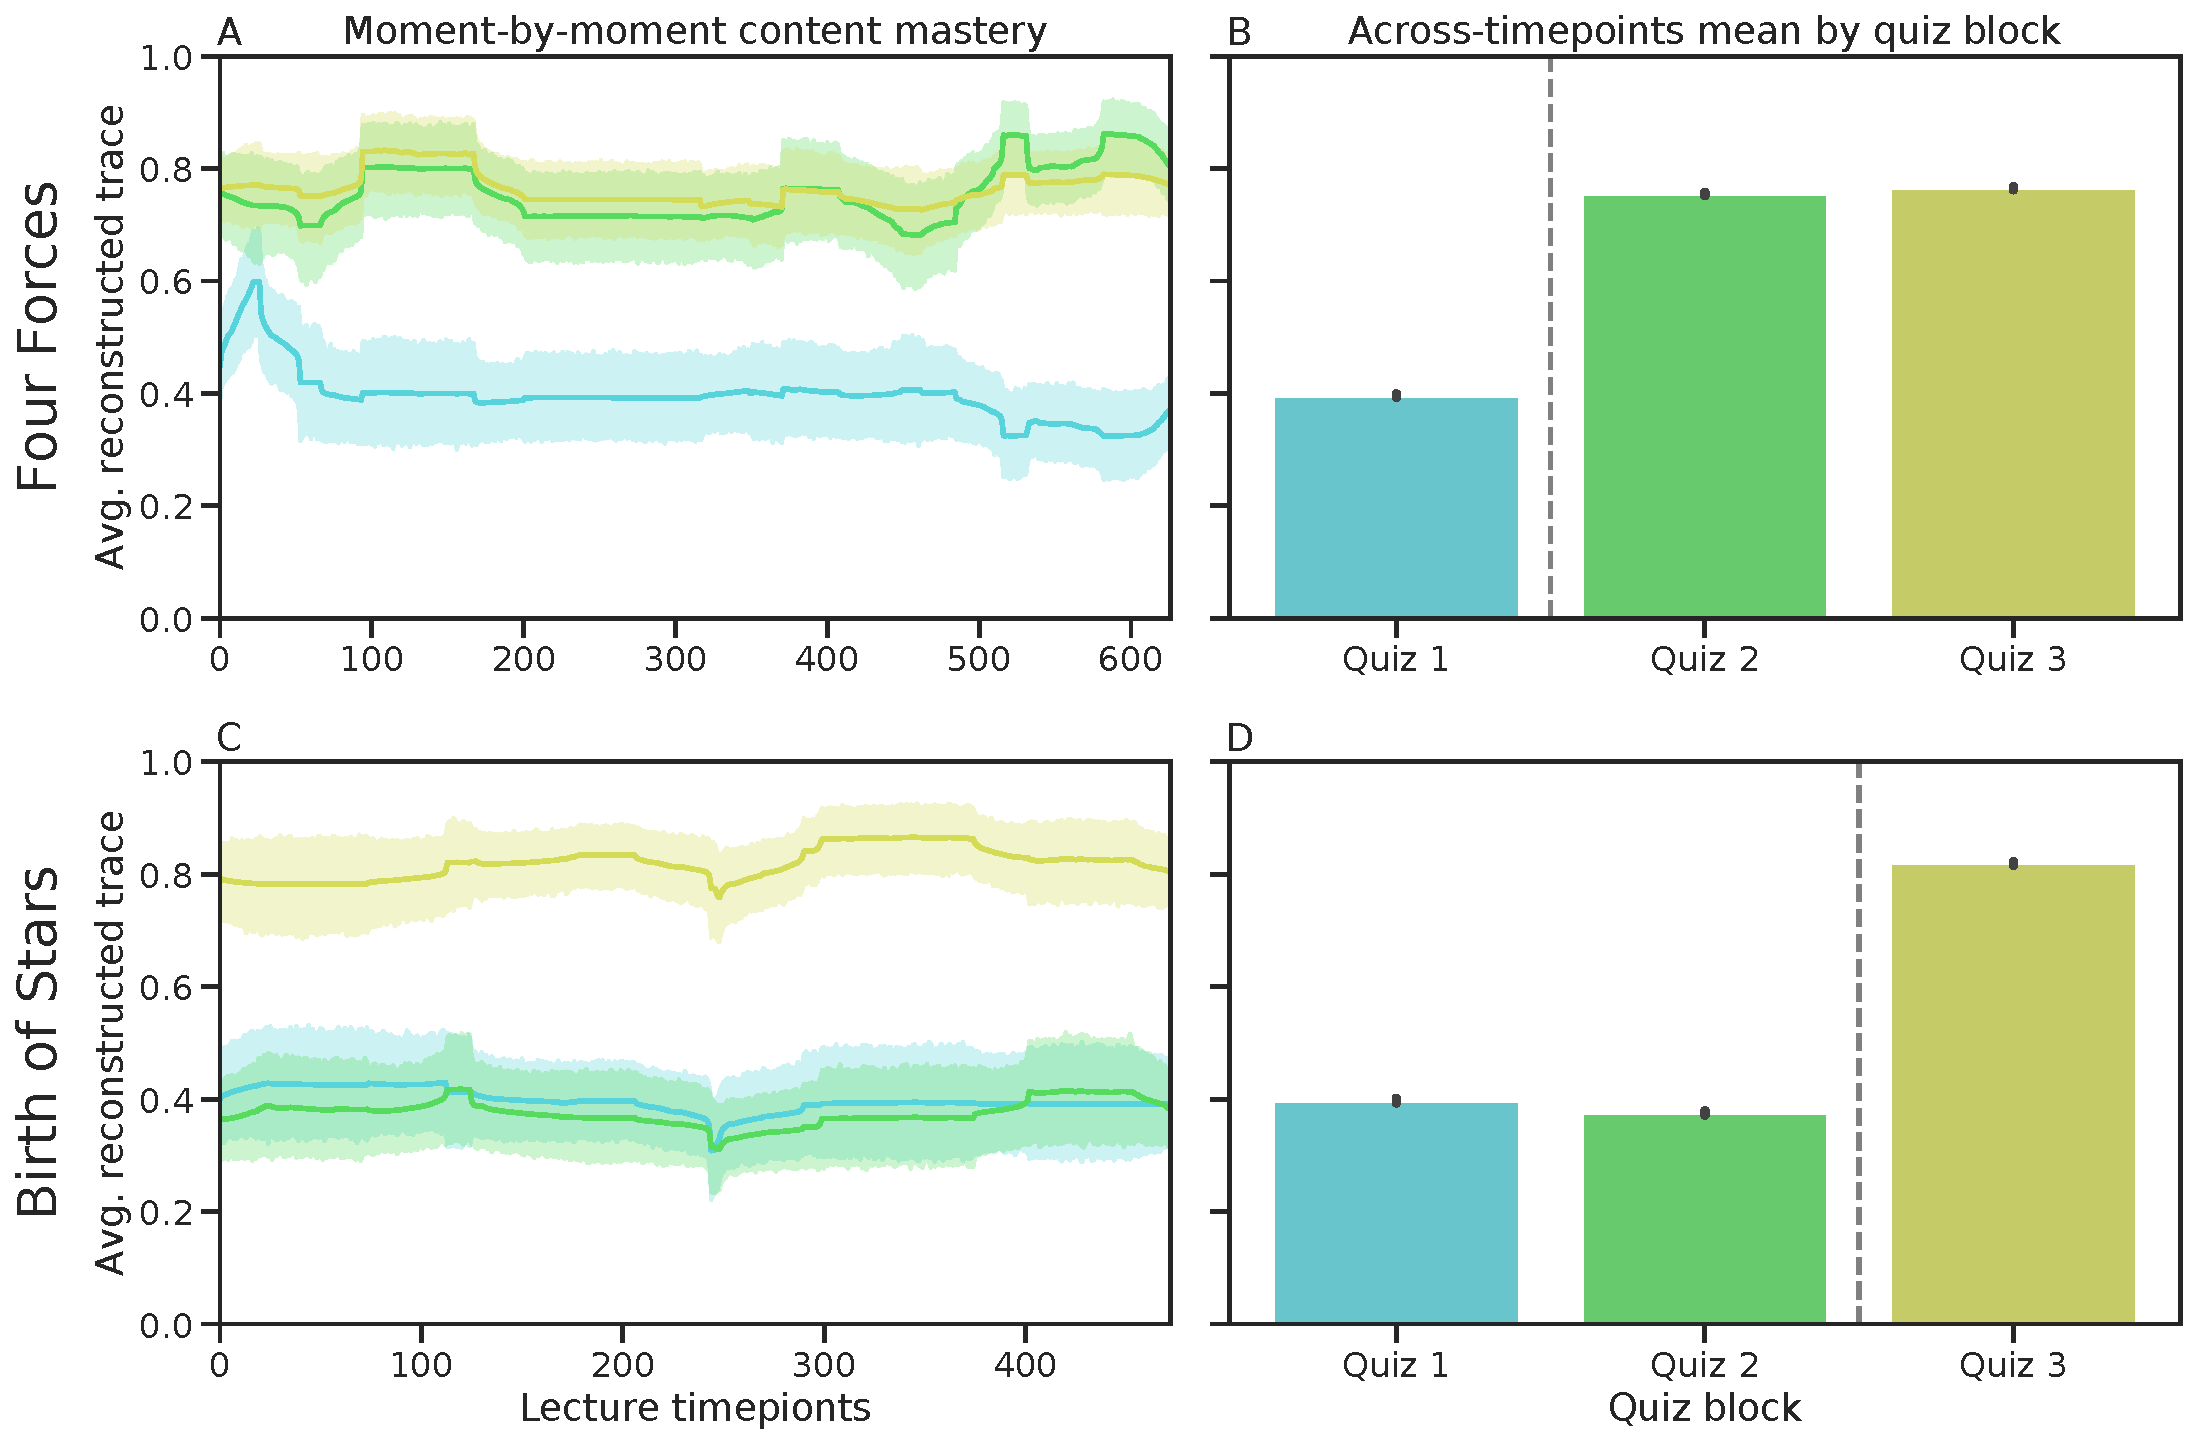
\includegraphics[width=0.8\textwidth]{figs/content-mastery}
% \caption{\textbf{Caption.} Placeholder text.}
% \label{fig:demo}
% \end{figure}

\section*{Discussion}

\section*{Materials and methods}

\subsection*{Participants}

We enrolled a total of 50 Dartmouth undergraduate students in our study.
Participants received course credit for enrolling. We asked each participant to
fill out a demographic survey that included questions about their age, gender,
native spoken language, ethnicity, race, hearing, color vision, sleep, coffee
consumption, level of alertness, and several aspects of their educational
background and prior coursework.

Participants' ages ranged from 18 to 22 years (mean: 19.52 years;
standard deviation: 1.09 years). A total of 15 participants reported
their gender as male and 35 participants reported their gender as
female. A total of 49 participants reported their native language as
``English'' and 1 reported having another native language. A total of
47 participants reported their ethnicity as ``Not Hispanic or Latino''
and three reported their ethnicity as ``Hispanic or Latino.''
Participants reported their races as White (32 participants), Asian
(14 participants), Black or African American (5 participants),
American Indian or Alaska Native (1 participant), and Native Hawaiian or
Other Pacific Islander (1 participant). (Note that some participants
selected multiple recial categories.)

A total of 49 participants reporting having normal hearing and 1
participant reported having some hearing impairment. A total of 49
participants reported having normal color vision and 1 participant
reported being color blind.  Participants reported having had, on the
night prior to testing, 2 -- 4 hours of sleep (1 participant), 4 -- 6
hours of sleep (9 participants), 6 -- 8 hours of sleep (35
participants), or $8+$ hours of sleep (5 participants). They reported
having consumed, on the same day and leading up to their testing
session, 0 cups of coffee (38 participants), 1 cup of coffee (10
participants), 3 cups of coffee (1 participant), or $4+$ cups of
coffee (1 participant).

No participants reported that their focus was currently impaired
(e.g., by drugs or alcohol).  Participants reported their current
level of alertness, and we converted their responses to numerical
scores as follows: ``very sluggish'' (-2), ``a little sluggish'' (-1),
``neutral'' (0), ``fairly alert'' (1), and ``very alert'' (2). Across
all participants, a range of alertness levels were reported (range: -2
-- 1; mean: -0.10; standard deviation: 0.84).

Particpants reported their undergraduate major(s) as Social Sciences
(28 participants), Natural sciences (16), Professional (e.g., pre-med
or pre-law; 8 participants), Mathematics and engineering (7
participants), Humanities (4 participants), or Undecided (3
participants).  Note that some participants selected multiple
categories for their undergraduate major.  We also asked participants
about the courses they had taken.  In total, 46 participants reported
having taken at least one Khan academy course in the past or being
familiar with the Khan academy, and 4 reported not having taken any
Khan academy courses.  Of the participants who reported having watched
at least one Khan academy course, 1 participant declined to report the
number of courses they had watched; 7 participants reported having
watched 1--2 courses; 11 reported having watched 3--5 courses; 8
reported having watched 5--10 courses; and 19 reported having watched
10 or more courses.  We also asked participants about the specific
courses they had watched, categorized under different subject areas.
In the ``Mathematics'' area participants reported having watched
videos on AP Calculus AB (21 participants), Precalculus (17
participants), Algebra 2 (14 participants), AP Calculus BC (12
participants), Trigonometry (11 participants), Algebra 1 (10
participants), Geometry (8 participants), Pre-algebra (7
participants), Multivariable Calculus (5 participants), Differential
Equations (5 participants, Statistics and Probability (4
participants), AP Statistics (2 participants), Linear Algebra (2
participants), Early Math (1 participant), Arithmetic (1 participant),
and other videos not listed in our survey (6 participants).  In the ``Science and engineering''
area participants reported having watched videos on Chemistry, AP
Chemistry, or Organic Chemstry (21
participants); Physics, AP Physics I, or AP Physics II (15 participants); Biology, AP
Biology; or High school Biology (15 participants); Health and Medicine
(1 participant); or other videos not listed in our survey (20 participants).  We also asked
participants if they had specifically seen the videos used in our
experiment.  When we asked about the \textit{Four Fundamental Forces}
video, 45 participants reported not having watched it before, 1
participant reported that they were not sure if they had watched it
before, and 4 participants declined to respond.  When we asked about
the \textit{Birth of Stars} video, 46 participants reported not having
watched it before and 4 participants declined to respond.  When we
asked participants about non-Khan academy online courses, they
reported having watched or taken courses on Mathematics (15
participants), Science and engineering (11 participants), Test
preparation (9 participants), Economics and finance (3 participants),
Arts and humanities (2 participants), Computing (2 participants), and
other categories not listed in our survey (18 participants).  Finally,
we asked participants about in-person courses they had taken in
different subject areas.  They reported taking courses in Mathematics
(39 participants), Science and engineering (38 participants), Arts and
humanities (35 participants), Test preparation (27 participants),
Economics and finance (26 participants), Computing (15 participants),
College and careers (7 participants), or other courses not listed in
our survey (6 participants).


\subsection*{Experiment}

We hand-selected two roughly 10-minute course videos from the Khan Academy
platform: \textit{The Four Fundamental Forces} (an introduction to gravity,
electromagnetism, the weak nuclear force, and the strong nuclear force;
duration: 10 minutes and 29 seconds) and \textit{Birth of Stars} (an
introduction to how stars are formed; duration: 7 minutes and 57 seconds). We
hand-wrote 39 multiple choice questions: 15 about the conceptual content of
\textit{The Four Fundamental Forces}, another 15 about the conceptual content
of \textit{Birth of Stars}, and 9 other questions that tested for general
conceptual knowledge about basic physics (covering material that was not
presented in either video). The full set of questions may be found in
Table~\questions.

\begin{figure}[tp]
\centering
\includegraphics[width=\textwidth]{figs/experiment}

\caption{\textbf{Experimental paradigm.} Participants alternate between
answering 13-question multiple choice quizzes and watching two Khan academy
videos. Each quiz contains a mix of 5 questions about lecture 1, 5 questions about lecture 2,
and 3 general physics knowledge questions. The specific questions reflected on
each quiz, and the orders of each quiz's questions, were randomized across
participants.}

\label{fig:experiment}
\end{figure}

Participants began the main experiment by answering a battery of 13 randomly
selected questions (chosen from the full set of 39). Then they watched the
\textit{The Four Fundamental Forces} video. Next, they answered a second set of
13 questions (chosen at random from the remaining 20 questions). Fourth,
participants watch the \textit{Birth of Stars} video, and finally they answered
the remaining 13 questions. Our experimental procedure is diagramed in
Figure~\ref{fig:experiment}. We used the experiment to develop and test our
computational framework for estimating knowledge and learning maps.

\subsection*{Analysis}

\subsubsection*{Constructing text embeddings of multiple videos and questions}

\subsubsection*{Estimating held-out conceptual knowledge}

\subsubsection*{Creating knowledge and learning map visualizations}



\bibliographystyle{apa}
\bibliography{CDL-bibliography/cdl}
\end{document}
